% Options for packages loaded elsewhere
\PassOptionsToPackage{unicode}{hyperref}
\PassOptionsToPackage{hyphens}{url}
%
\documentclass[
]{article}
\usepackage{amsmath,amssymb}
\usepackage{iftex}
\ifPDFTeX
  \usepackage[T1]{fontenc}
  \usepackage[utf8]{inputenc}
  \usepackage{textcomp} % provide euro and other symbols
\else % if luatex or xetex
  \usepackage{unicode-math} % this also loads fontspec
  \defaultfontfeatures{Scale=MatchLowercase}
  \defaultfontfeatures[\rmfamily]{Ligatures=TeX,Scale=1}
\fi
\usepackage{lmodern}
\ifPDFTeX\else
  % xetex/luatex font selection
\fi
% Use upquote if available, for straight quotes in verbatim environments
\IfFileExists{upquote.sty}{\usepackage{upquote}}{}
\IfFileExists{microtype.sty}{% use microtype if available
  \usepackage[]{microtype}
  \UseMicrotypeSet[protrusion]{basicmath} % disable protrusion for tt fonts
}{}
\makeatletter
\@ifundefined{KOMAClassName}{% if non-KOMA class
  \IfFileExists{parskip.sty}{%
    \usepackage{parskip}
  }{% else
    \setlength{\parindent}{0pt}
    \setlength{\parskip}{6pt plus 2pt minus 1pt}}
}{% if KOMA class
  \KOMAoptions{parskip=half}}
\makeatother
\usepackage{xcolor}
\usepackage[margin=1in]{geometry}
\usepackage{graphicx}
\makeatletter
\def\maxwidth{\ifdim\Gin@nat@width>\linewidth\linewidth\else\Gin@nat@width\fi}
\def\maxheight{\ifdim\Gin@nat@height>\textheight\textheight\else\Gin@nat@height\fi}
\makeatother
% Scale images if necessary, so that they will not overflow the page
% margins by default, and it is still possible to overwrite the defaults
% using explicit options in \includegraphics[width, height, ...]{}
\setkeys{Gin}{width=\maxwidth,height=\maxheight,keepaspectratio}
% Set default figure placement to htbp
\makeatletter
\def\fps@figure{htbp}
\makeatother
\setlength{\emergencystretch}{3em} % prevent overfull lines
\providecommand{\tightlist}{%
  \setlength{\itemsep}{0pt}\setlength{\parskip}{0pt}}
\setcounter{secnumdepth}{5}
\usepackage{graphics}
\usepackage{amsmath, amsfonts, amsthm, amssymb, amscd,a4wide}
%\usepackage{algorithm}
% \usepackage{algpseudocode}
\usepackage{algorithmic}
\usepackage[linesnumbered,ruled,vlined]{algorithm2e}
\usepackage{hyperref}
\usepackage{url}
\usepackage{float}
\usepackage{epstopdf}
\usepackage{subcaption}
\let\oldmarginpar\marginpar
\renewcommand\marginpar[1]{\-\oldmarginpar[\raggedleft\footnotesize #1]%
{\raggedright\footnotesize #1}}


\floatname{algorithm}{Algorithm}
\renewcommand{\algorithmicrequire}{\textbf{Input:}}
\renewcommand{\algorithmicensure}{\textbf{Output:}}
\newcommand{\barrer}[1]{%
    \tikz[baseline] {
        \node[inner sep=0pt, outer sep=0pt, anchor=base] (X) {\strut#1}; 
        \draw[red, thick] (X.west) -- (X.east);
    }
}
%\usepackage[linesnumbered,ruled]{algorithm2e}

%%

% ces lignes permet de ne pas mettre en couleurs les liens hypertextes dans le fichier PDF
% cependant il est toujours possible de cliquer dessus
%

\usepackage{xcolor} %package pour les couleurs
\usepackage{tikz} % package principal TikZ
\usetikzlibrary{arrows} %librairieoptionnelle PGF
\usepackage{adjustbox}

\usepackage{slashed}
\usepackage{amsmath}
\usepackage{xcolor}
\usepackage{hyperref}
\hypersetup{linktoc = all}                % hyperref settings
%\hypersetup{pdfborderstyle={/S/U/W 0.5}}  % hyperref settings
\hypersetup{hidelinks}
\hypersetup{bookmarksnumbered}
\pdfstringdefDisableCommands{%
  \def\({}%
  \def\){}%
  \def\\{}%
  \def\infty{\042\036}%
  \def\Tr{Tr }%
}
%%%%%%%%% 
\newtheorem{definition}{Definition}[section]
\newtheorem{corollary}[definition]{Corollary}
\newtheorem{lemma}[definition]{Lemma}
\newtheorem{theorem}[definition]{Theorem}
\newtheorem{proposition}[definition]{Proposition}
\newtheorem{theoremdefinition}[definition]{Theorem and Definition}
\newtheorem{remark}[definition]{Remark}
\newtheorem{conjecture}{Conjecture}
\newtheorem{HP}{Highlighted point}
% 
\numberwithin{equation}{section}
\newcommand\norm[1]{\left\lVert#1\right\rVert}
\newcommand \be   {\begin{equation}}
\newcommand \bel {\begin{equation}\label}
\newcommand \ee   {\end{equation}}
\newcommand \dist {{\mbox{\em dist }}}
\newcommand \sgn {{\text{sgn }}}
\newcommand \meas {{\text{meas }}}
\newcommand \supp {{\text{supp }}}
\newcommand \Id   {{\text{Id}}}
\newcommand \smin {s^{\text{min}}}
\newcommand \smax {s^{\text{max}}}
\newcommand \lmin {{\lam^{\text{min}}}}
\newcommand \lmax {{\lam^{\text{max}}}}
\newcommand \RR    {\mathbb{R}}
\newcommand \NN    {\mathbb{N}}
\newcommand \ZZ    {\mathbb{Z}}
\newcommand \QQ    {\mathbb{Q}}
\newcommand \PP    {\mathbb{P}}
\newcommand \EE    {\mathbb{E}}
\newcommand \Rp    {\mathbb{R}^\plus }
\newcommand \RRR    {\mathbf{R}}
\newcommand \SSS    {\mathbf{S}}
\newcommand \Scal    {\mathcal{S}}
\newcommand \Pcal    {\mathcal{P}}
\newcommand \Tbar {\overline T}
\newcommand \Acal {\mathcal A}
\newcommand \Bcal {\mathcal B}
\newcommand \Ccal    {\mathcal{C}}
\newcommand \Mcal    {\mathcal{M}}
\newcommand \Lcal    {\mathcal{L}}
\newcommand \Jcal    {\mathcal{J}}
\newcommand \Kcal    {\mathcal{K}}
\newcommand \Wbf {\mathbf W}
\newcommand \Hcal    {\mathcal{H}}
\newcommand \Tcal    {\mathcal{T}}
\newcommand \lam   {\lambda}
\newcommand \sig   {\sigma}
\newcommand \gam   {\gamma}
\newcommand \ubar   {\overline u}
\newcommand \HH    {\mathcal{H}}
\newcommand \CC    {\mathcal{C}}
\newcommand \Ncal    {\mathcal{N}}
\newcommand \DDD    {\mathcal{D}}
\newcommand \RN    {{\RR^N}}
\newcommand \eps   {\epsilon}
\newcommand \Lam   {\Lambda}
\newcommand \BB    {{\mathcal B}}
\newcommand \WW    {{\mathcal W}}
\newcommand \MM    {{M}}
\newcommand \AAA    {{\mathcal A}}
\newcommand \JJ    {{\mathcal J}}
\newcommand \II    {{\mathcal I}}
\newcommand \LLL    {{\mathbf L}}
\newcommand \VVV    {{\mathbf V}}
\newcommand \QQQ    {{\mathbf Q}}
\newcommand \Rd    {{\mathbb{R}^d}}
\newcommand \CCD    {{\mathbb{C}^D}}
%
\newcommand \del   {\partial}
\newcommand \blam  {{\underline\lambda}}
\newcommand \lamb  {{\overline\lambda}}
\newcommand \Bzero    {{\mathcal{B}_{\delta_0}}}
\newcommand \Bone    {{\mathcal{B}_{\delta_1}}}
\newcommand \Btwo    {{\mathcal{B}_{\delta_2}}}
\newcommand \la         \langle
\newcommand \ra     \rangle
\newcommand \ab     {\overline a}
\newcommand \mmm  {p}

\newcommand \Ybf {\mathbf Y} 
\newcommand \Sbf {\mathbf S} 
\newcommand \hbf {\mathbf h} 

\newcommand \Sbar {\overline S}
\newcommand \Aund {\underline{\Acal}}
\newcommand \Aove {\overline{\Acal}}

\newcommand \plus {+}

\newcommand \RD {{\mathbb R}^D}


\usepackage{mathrsfs}

%*************************************************************************************
\usepackage{authblk}


\setcounter{Maxaffil}{0}
\renewcommand\Affilfont{\itshape\small}




\urlstyle{same}
\hypersetup{
  hidelinks,
  pdfcreator={LaTeX via pandoc}}

\date{\vspace{-2.5em}}

\title{\textbf{Professionnal Capstone}}
\author[1]{Aguirre Max}
\affil[1]{PSTB, Paris, France}

\date{\today} % Current date, or specify manually

\begin{document}

\maketitle % Generate title

\begin{abstract}
Current Deep Learning frameworks and architecture lack explainability and reproductibility, which can lead to significant issues in some domains, for instance in finance, where understanding model decisions is crucial for compliance and risk management \cite{??}. In this document, we propose a self-contained, detailed, description of a scalable standardized kernel (RKHS) approach to popular reinforcement learning algorithms, where agents interact with environments having continuous states and discrete actions spaces, dealing with possibly unstructured data. These algorithms, namely Q-Learning, Actor Critic, Q-Value Gradient, Hamilton-Jacobi-Bellman (HJB) and Heuristic Controls, are implemented with a RKHS library \cite{codpy} using default settings. We show that this approach to reinforcement learning is accurate, robust, sample efficient and versatile, as we benchmark our algorithms in this paper on simple games and use them as a baseline for our applications.
\end{abstract}

\noindent\textbf{Keywords:} Reinforcement Learning, Q-Learning, Actor Critic, RKHS, Kernel Methods, Hamilton-Jacobi-Bellman, Heuristic Controls

\hypertarget{Introduction}{%
\section{Introduction}\label{Introduction}}

Reinforcement Learning (RL) is a powerful framework for sequential decision-making, where agents learn optimal behaviours by interacting with an environment \cite{sutton2018}. This environment is usually modelled as a Markov Decision Process (MDP) $\mathcal{M} = (\mathcal{S}, \mathcal{A}, R, P)$, where an agent seeks to learn a policy 
$\pi$ that maximizes the value function, usually taken as the expected cumulative reward over time. Traditional RL algorithms, such as Q-learning \cite{watkins1992} and policy gradient methods \cite{silver2014}, rely on function approximators to estimate value functions. Deep neural networks (DNNs) are widely used as function approximators.  

However, function approximation using DNNs in RL is challenging due to issues such as catastrophic forgetting, instability \cite{vanhasselt2016}, performance issues, and the need for extensive hyperparameter tuning \cite{mnih2015} as well as they suffer from high sensitivity to initialization, overfitting, and lack of convergence guarantees.

An alternative approach is to use kernel-based methods, which offer function approximation with well-defined theoretical properties.  The application of kernel methods in RL has been explored in various contexts. Kernel regression for Q-function approximation was proposed in \cite{ormoneit2002}, while Gaussian Processes were introduced for value function estimation in \cite{engel2003}, leading to Gaussian Process Temporal Difference Learning (GPTD). Additionally, methods based on Reproducing Kernel Hilbert Space (RKHS) for policy gradient estimation were studied in \cite{Xu2007}, and recent theoretical bounds have been established in \cite{SF2023}. Despite their theoretical advantages, kernel methods remain underutilized in RL due to computational complexity, scalability limitations, lack of RKHS dedicated software frameworks and analysis. 

Numerical kernel methods for Hamilton–Jacobi–Bellman (HJB) equations, a topic closely related to reinforcement learning, have a long history in mathematical finance, see \cite{PLF-JMM-Wilmott} and references therein. Indeed, there is a straightforward correspondence between reinforcement learning and financial decision problems, where rewards and states in RL relate to payoffs and risk factors in finance. HJB equations arise in option pricing, investment strategies, market making, or optimal execution. This paper can thus be seen as an exploration of kernel-based decision technologies, inspired by financial applications, to tackle reinforcement learning problems.

This paper aims to popularize RKHS reinforcement learning approaches proposing a standardized and scalable analysis to reinforcement learning that systematically integrate kernel-based regression techniques to improve value function estimation and policy optimization. Specifically, the contributions of this work are as follows:

\begin{itemize}
\item A standardized kernel analysis to reinforcement learning for value function estimations and Bellman residuals. This analysis includes any RKHS approaches, as Gaussian processes, Gaussian mixture, etc...

\item A robust kernel implementation to popular algorithms: Q-Learning, Actor-Critic, Q-Value Gradient, HJB, and heuristic control learning.

\end{itemize}

This kernel approach is implemented using a standard RKHS library \cite{codpy}, facilitating accessibility and reproducibility for researchers and practitioners. We focus in this paper on small to medium dataset, but the library \cite{codpy} provide tools to scale up if needed, see \cite{LeMeMi:2024}. We experiment clustered versions of these algorithms in this paper, which enhance scalability and efficiency.

The remainder of this paper is organized as follows. In Section \ref{Background}, we introduce the fundamental principles of RL, covering the agent-environment interaction, reward mechanisms, and the Bellman equations, along with classical RL algorithms such as Q-learning, Q-Value Gradient methods, heuristic-controlled learning, and Hamilton-Jacobi-Bellman. Section \ref{Kernel Reminder} provides the strict required knowledge concerning kernel methods, detailing function approximation in RKHS, kernel-based regression, gradient estimation techniques and conditional probability estimations as well as notations, in order to formulate our approach. In Section \ref{Kernel RL Algorithms}, we present our kernelized reinforcement learning framework, systematically adapting standard RL methods, including kernelized Q-learning, Q-value gradient estimation, actor-critic with Bellman residual advantage, heuristic-controlled learning and Hamilton-Jacobi-Bellman. Section \ref{Experiments} evaluates our framework on benchmark environments, comparing its performance with the popular Deep Q-Network, see \cite{DQN}, and PPO \cite{PPO}, that are our best algorithms at hand to handle our numerical experiments.


\hypertarget{Background}{%
\section{Background}\label{Background}}

\hypertarget{Reinforcement-learning}{%
\subsection{Reinforcement Learning}\label{Reinforcement-learning}}

\hypertarget{General framework for RL}{%
\subsubsection{General Framework for RL}\label{General framework for RL}}

In reinforcement learning (RL), an \emph{agent} interacts with an
\emph{environment}, over discrete time steps. At each time step \(t\),
the agent observes the current state \(s_t \),
selects an action \(a_t\),
and receives a \emph{reward} signal \(r_t \) along with the
\emph{next state} \(s_{t+1}\) from the environment. 

We will use Markov Decision Process (MDP) framework which is defined as a tuple
\(\mathcal{M} = (\mathcal{S}, \mathcal{A}, R, P)\), where \(\mathcal{S} \subset \mathbb{R}^D\) is the set of all valid states, \(\mathcal{A}\) is a discrete set of all valid actions, \(R : \mathcal{S} \times \mathcal{A} \rightarrow \mathbb{R}\) is the environment reward function, which provides the reward obtained from taking an action in a given state (\(r_t = R(s_t, a_t)\)) and \(S : \mathcal{S} \times \mathcal{A} \rightarrow \mathcal{S}\) is the environment next state function, which determine the
next states obtained from taking an action in a given state (\(s_{t+1} = S(s_t, a_t)\)).

The rewards and the next state function can be either deterministic or
stochastic, in latter case there exist joint probability law
\(\mathbb{P}_R : \mathcal{S} \times \mathcal{A} \rightarrow \mathbb{P}(R)\),
\(\mathbb{P}_S : \mathcal{S} \times \mathcal{A} \rightarrow \mathbb{P}(\mathcal{S})\),
which determine the likelihood of receiving a reward
\(r'\) and transitioning to a state \(s'\) from \(s \in \mathcal{S}\) after taking
action \(a \in \mathcal{A}\): \begin{equation}\label{tran}
\mathbb{P}_S(s_{t+1} = s' \mid s_t = s, a_t = a), \quad \mathbb{P}_R(r_{t+1} = r' \mid s_t = s, a_t = a)
\end{equation} 
By abuse of notation, we make no distinction between observed rewards
\(r_t=R(s_t,a_t)\) and their expectations
\(\mathbb{E}[R |s_t, a_t]\). This allows us to simplify the notation by assuming a deterministic reward structure, although we will consider the stochastic case for states transitions while describing HJB equations.

MDP assume the
Markov property, which means the future state depends only on the
current state and action, not on the sequence of events that preceded
it. However, we emphasize that the numerical analysis developed in this paper holds beyond Markov assumptions.

The goal of RL is to learn a
policy \(\pi\) that maximizes the cumulative discounted reward, or
\emph{return} \(G_t = \sum_{k=t}^{T_e} \gamma^{k-t} r_k\) at time \(t\),
where \(0 \le \gamma \le 1\) is a discount factor and \(T_e\) is the number of time steps for episode $e$. 

The
\emph{policy} \(\pi(s)=(\pi^1,\dots,\pi^{|\mathcal{A}|})(s)\) is a
probability field describing an agent, determining its actions according to a
probability depending on the states of the environment. This setting
includes both stochastic or deterministic policies, in which later case
$\pi^a(s_t) = \delta^a(a_t)$, where the Kronecker $\delta$ function is defined as $\delta^i(j) = \{1 \text{ if } i=j; 0 \text{ else} \}$.

Our numerical experiments deal with learning in the following sense: our agents define a new policy $\pi^{e+1}(\cdot)$ analysing all past $e$ episodes, and this policy is used in the next game episode $e+1$, covering both online and offline learning.

Let us introduce the buffer, that is the memory of past $e$ games episodes as a collection of stored
trajectory, denoted \( B^{T^e} = \{(s_t^e, a_t^e, s_{t+1}^e, r_t^e, d_t^e) \}_{t=1}^{T^e}\) : states, actions, next states, rewards, dones, the last being a Boolean to indicate if the next state is terminal, corresponding to data terminating a game session. We need this notation for heuristic control, based on episodes, however we consider and note the input data as unordered, possibly unstructured data as buffers \( B^{T} = \{(s_t, a_t, s_{t}', r_t, d_t) \}_{t=1}^{T} \) for kernel bellman error based algorithms (QLearning, Actor Critic, $Q$-Value Gradient and HJB).


\hypertarget{Bellman Equations}{%
\subsubsection{Bellman Equations}\label{Bellman Equations}}

We now introduce the main definition relative to value and state-action value function and their respective Bellman equations: 

\textbf{The state-value function} \(V^{\pi}\) of a MDP is the expected
return starting from a given state \(s\) and following policy \(\pi\),
i.e. \begin{equation}
V^{\pi}(s) = \mathbb{E}^{\pi} \left[ G_t \mid s_t = s \right] = \mathbb{E}^{\pi} \left[ R(s,\cdot) + \gamma V^{\pi}(s') \mid s_t = s \right]
\label{valfun_bell}
\end{equation}

where $s'=S(s,\cdot)$.
This is a recursive definition that coincides to the return computation of the last played game ($V^{\pi}(s_t) = G_t$) with a deterministic policy and environment.

\textbf{The state-action-value function} \(Q^{\pi}\) measures the
expected return starting from \(s\), taking action \(a\), and following
policy \(\pi\): \begin{equation}
Q^{\pi}(s,a) = \mathbb{E}^{\pi} \left[ G_t \mid s_t = s, a_t = a \right] = R(s,a) + \gamma \mathbb{E}^{\pi} \left[  Q^{\pi}(s',a) \mid s_t = s, a_t = a \right]
\label{sta_act_valfun}
\end{equation}

\textbf{The optimal state-value function} \(V^{\pi^*}(s)\) represents the expected return when starting in state \(s\) and consistently following the optimal policy $\pi^*$ within the environment: \begin{equation}
 V^{\pi^*}(s) = \arg \max_{\pi} V^{\pi}(s) 
\label{opt_valfun}
\end{equation} \textbf{The optimal state-action-value function}
\(Q^{\pi^*}(s,a)\) represents the expected return when starting in state
\(s\) and acting a, and following the optimal policy in the environment, satisfying
\begin{equation}
Q^{\pi^*}(s,a) = \arg \max_{\pi} Q^{\pi}(s,a)
\label{opt_sta_act_valfun}
\end{equation}


The value functions estimates should satisfy Bellman equation to allow policy improvement. This is the backbone of a class of reinforcement
learning algorithms called \textbf{value-based methods}. 
On
the other hand we have \textbf{policy-based methods} which goal is to
directly approximate the optimal policy \(\pi^*\).



\hypertarget{Algorithms}{%
\subsection{Algorithms}\label{Algorithms}}

\hypertarget{Q-learning}{%
\subsubsection{Q-learning}\label{Q-learning}}


One of the most prominent value-based algorithms is Q-learning, which
aims to learn the optimal state-action-value function, \(Q^{\pi^*}(s,a)\). 
The core idea
of Q-learning is to solve the optimal Bellman equation \eqref{opt_sta_act_valfun}. For instance, a popular iterative scheme is given by the following iterative rule: 
\begin{equation} 
Q^{\pi_{n+1}}(s_t,a_t) = Q^{\pi_{n}}(s_t,a_t) + \alpha[R(s_{t},a_t) + \gamma \max_{a} Q^{\pi_{n}}(s_{t+1},a) -Q^{\pi_{n}}(s_t,a_t)],
\label{iter_bell}
\end{equation} where $\alpha$ is a learning rate. Once iterated $N$ times, the so called \textit{greedy} policy corresponds to choosing in-game actions according to $\text{argmax}_{a \in \mathcal{A}} Q^{\pi_{N}}(s,a)$.
Such deterministic strategies can limit state space exploration, so reinforcement learning algorithms use techniques like the epsilon-greedy strategy to balance exploration and exploitation for effective learning.

Let us have a look to the structure of the scheme \eqref{iter_bell}. This scheme exploits the Markov properties of environments, leveraging the time structure of the buffer data, and can be described as a \textit{backward} time-evolution equation, allowing for numerous optimization techniques. By contrast, in this paper, we provide a numerical analysis that holds beyond Markov assumptions, trading optimization for generality, and unstructured data, that is considering $s'_t$ instead of $s_{t+1}$ in \eqref{iter_bell}.

\hypertarget{Policy Gradient}{%
\subsubsection{Policy Gradient}\label{Policy Gradient}}

Policy gradient methods aim to optimize a policy by directly calculating the gradient of a scalar performance measure with respect to the policy parameters.  These methods fall into two categories: those that directly approximate the policy, and actor-critic methods, which approximate both the policy and the value function.

The general rule can be written as follows: \begin{equation}
 \pi_{n+1}(s) = \pi_n(s) + \lambda A^{\pi_n}(s), 
\label{PG_rule}
\end{equation}


Where \( \lambda \) is a learning rate, and \( A^{\pi}\) is a vector field with components \( A^{\pi} = \{A^{1,\pi}, \dots, A^{|\mathcal{A}|,\pi}\} \), under the constraint that the equation \eqref{PG_rule} defines a probability \( \pi_{n+1} \propto \pi_n e^{\lambda A^{\pi_n}} \). The equation \eqref{PG_rule} can be interpreted in the continuous time case as: \( \frac{d}{dt} \pi_t(s) = \lambda A^{\pi_t}(s) \). We focus on two cases. 


\begin{itemize}
\item 
The first case is reminiscent of policy gradient methods, where the update aims to improve the value function:
\begin{equation} \label{eq:advant1}
A^{\pi}(s) = \nabla_{\pi} V^{\pi}(s).
\end{equation}
 
\item 
The second case corresponds to standard actor-critic methods, tailored to minimize the Bellman residuals:
\begin{equation} \label{eq:advant2}
 A^{\pi^a}(s) = R(s,a) + \gamma V^{\pi}(s') - V^{\pi}(s), \quad s'=S(s,a).
\end{equation}
\end{itemize}

From a numerical point of view, a common approach is to use a set of parameters \( \theta \) to describe policies \( \pi_n(s) = \pi(s,\theta_n) \), so that \eqref{PG_rule} usually transform into an evolution equation of the parameters \( \theta_{n+1} \leftarrow f(\theta_n)\), where \( f \) depends on the used regression methods. 

\subsubsection{HJB Equation}\label{HJB}

We describe an approach inspired from HJB equation.
This approach relies on the model of the next state function, split into two terms, the first one capturing the deterministic part, the other capturing a conditional noise defining a local martingale. For instance, consider the following model:

\begin{equation}\label{HJBEq}
 s_{t+1} = S_\epsilon(s_t,a_t),\quad S_\epsilon(s_t,a_t)=s_t+F(s_t,a_t)+\epsilon | s_t,a_t,
\end{equation}
where $(\epsilon | s_t,a_t)$ is a conditional noise, and $F(s_t,a_t) = \mathbb{E}[s_{t+1} | s_t,a_t] - s_t$ is a conditional expectation which is a continuous function of $(s_t,a_t)$. The choice of $\epsilon$ depends on the problem context, but it is typically chosen to approximate white noise. This setting defines the value function as solution of
\begin{equation}
Q^{\pi}(s_t,a_t) = R(s_t,a_t) +  \gamma \mathbb{E}^{\pi,s'}\left[Q^{\pi}(s',\cdot) \mid s_t,\cdot\right].
\end{equation}
Thz last expression can be better understood using transition probabilities
\begin{equation}
Q^{\pi}(s_t,a_t) = R(s_t,a_t) +  \gamma   \int \left[ \sum_{a \in \mathcal{A}} \pi^a(s_t) Q^{\pi}(s',a)\right] d \mathbb{P}_S(s',s_t,a_t),
\end{equation}
where $ d \mathbb{P}_S(s' \mid s,a)$ represents the probability measure of transitioning from state $s$ to state $s'$ given action $a$ introduced in \eqref{tran}.
Solving the previous equation for $Q^\pi$ involves thus estimating the conditional expectation $F(s,a)$, as well as the transition probability measure $d \mathbb{P}_S$. The last transition probability is usually estimated assuming that the noise $\epsilon$ is a white noise having Gaussian structure, but the section \ref{KHJB} proposes methods that solves \eqref{HJB} without assumptions on the conditional noise $\epsilon | s_t,a_t$.

\hypertarget{Heuristic-Controlled Learning}{%
\subsubsection{Heuristic-Controlled Learning}\label{Heuristic-Controlled Learning}}

A controller is a deterministic policy parametrized by a set of parameters $\theta$, \( \mathcal{C}^{\theta} : \mathcal{S} \rightarrow \mathcal{A} \),
for \( \theta \in \Theta \), with $\Theta$ being a bounded, closed and convex set, where each $\theta$ defines an agent's behaviour. At the beginning of each episode $e$, the agent selects $\theta_e$, the parameters for that episode, where $e$ is the episode index. The agent then observes $r_e$, a function of rewards collected during episode $e$, typically defined as the mean of rewards across the episode. The objective is to maximize $\mathbb{E}[r|\theta]$. 

This setting is like a continuous black-box optimization problems, rather than classical reinforcement learning problem, as it is non-associative:  the learned behaviour is not tied to specific states of the environment. Only episode-level rewards $r_e$ are observed. 
The actions space $\Theta$ is continuous, and there are no concerns of Bellman equations, buffer and transitions. However we make a strong assumption assuming that the expectation of the rewards $\mathbb{E}[r|\theta]$ is continuous in $\theta$.

We introduce a model, $R_e(\theta) \sim \mathbb{E}[r|\theta]$, designed to estimate  the conditional expectation of rewards $r$ given $\theta$ based on the first $e$ observations $r_1, \dots, r_e$ and $\bar{\theta_e} = \{ \theta_1, \cdots, \theta_e \}$. 
We consider an optimization function $\mathcal{L}(R_e,\theta)$ and we solve iteratively on each game episode
\begin{equation}
 \theta_{e+1} = \text{argmax}_{\theta \in \Theta} \mathcal{L}(R_e,\theta)
 \label{HCEq}
\end{equation}

There are multiple choices to pick the functional $\mathcal{L}$, all motivated by providing an exploration incentive. For instance, we experienced that
\begin{equation}\label{hc_model}
\mathcal{L}(R_e,\theta) = \big( R_e(\theta) - \min_{\bar{\theta_e}}(R_e(\theta)) \big) d(\theta, \bar{\theta_e}),
\end{equation}where $d(\theta, \bar{\theta_e})$ is the kernel-induced distance gives satisfactory results, but another potential choice is given by $\mathcal{L}(R_e,\theta) = R_e(\theta) - \sigma_e(r|\theta)$ where $\sigma_e(r|\theta)$ is an estimator of the conditional variance of the law $r|\theta$. Note that this is reminiscent of Upper Confidence Bound (UCB) approach, however the context here is different as we assume continuity in conditional expectations.


This family of problems are paramount for applications: in several situations one can achieve far better results with a good controller than with Bellman-residual approaches on common reinforcement learning tasks, and the same setting applies also to other problems as hyperparameter tuning or PID controllers. Notice however that an expert-knowledge controller is not always available, and no clear way to automatically define one exists to our knowledge. However, due to the importance of these approaches, we propose a kernel method to solve \eqref{HCEq} in section \ref{Heuristic-controlled Learning}.

\hypertarget{Kernel Reminder}{%
\subsection{Kernel Reminder}\label{Kernel Reminder}}
\paragraph*{Positive Definite Kernels} A function \(k: \RR^D \times \RR^D \mapsto \mathbb{R}\) is
called a \textit{kernel} if it is symmetric and positive definite (see
\cite{BTA} for a definition). Given two sets of points
\(X \in \RR^{N_X,D}\) and \(Y \in \RR^{N_Y,D}\), we introduce their
associated \textit{kernel matrix} \begin{equation}
K(X,Y)= \big\{k(x^i,y^j)\big\}^{i,j} \in \mathbb{R}^{N_X,N_Y}.
\end{equation} 
An important property of positive-definite kernels is to define symmetric, positive-definite kernel matrices \(K(X,X)\), called Gram matrices, which are invertible
provided \(X\) consists of \textit{distinct} points in \(\RR^{N_X,D}\).

\paragraph*{Kernel-Based Function Approximation}
Given a set \(X\), a kernel defines a space of vector-valued functions (regressors), in which functions are parametrized by
matrices $\theta$ in \(\mathbb{R}^{N_X,D_f}\), as follows: 
\begin{equation}
\label{Hk}
\mathcal{H}_k^X = \Big\{f_{k,\theta}(\cdot) = \sum_{n=1}^{N_X} \theta^n k(\cdot,x^n) = K(\cdot,X) \theta, \quad \theta \in \mathbb{R}^{N_X,D_f} \Big\}.
\end{equation} Here, the parameters \(\theta\) are computed,
or \textit{fitted}, to a given continuous function $f(\cdot) \in \mathbb{R}^{D_f}$, described by discrete values \(Y,f(Y)\), commonly referred as a training set, according to the relation
\begin{equation}\label{FIT}
 f_{k, \theta} (\cdot) = K(\cdot,X) \theta, \quad \theta = \Big( K(Y,X) + \epsilon R(Y,X) \Big)^{-1} f(Y),
\end{equation} in which \(\epsilon \ge 0\) and \(R(Y,X)\) determine an
optional regularizing term. All along this paper, matrix inversion as in \eqref{FIT}  are computed using a least-square method, although other methods could be considered. We use the notation $f_{k}$ for short to denote kernel regression, but depending on context, we disambiguate our choices of parameters with $f_{k, \theta}$. 


\paragraph*{Operator View and Gradient Estimation} Consider $Y=X$ from here for simplicity. Ridge regression uses Tikhonov regularization, corresponding to $R$ taken as the identity matrix. The above fitting procedure can be also
expressed as an operator \(\mathcal{P}_k\) and a scalar product or a matrix multiplication:
\begin{equation}\label{OP}
 f_{k}(\cdot) = \mathcal{P}_k(\cdot,X) f(X), \qquad \mathcal{P}_k(\cdot,X) =K(\cdot,X)\big( K(X,X) + \epsilon R(X,X) \big)^{-1},
\end{equation} 
$\mathcal{P}_k(\cdot,X)$ being a vector of length $N_X$. This operator standpoint allows to define the kernel-based
\textit{gradient operator} as \begin{equation}
\label{nabla}
 \nabla f_{k}(\cdot) = \nabla_k(\cdot) f(X), \quad \nabla_k(\cdot) = (\nabla K)(\cdot,X)\big( K(X,X) + \epsilon R(X,X) \big)^{-1}.
\end{equation}

\paragraph*{Kernel-Based Estimation of Conditional Expectations} Let us now turn to the statistical point of view : consider $f(\cdot)$ a noisy function, known from observations $X,f(X)$, where $X$ are i.i.d samples of a distribution $\mathbb{X}$ having density $\pi(\cdot)$. The celebrated Nadaraya-Watson approach, dating back to the 1960's, give a classical estimator of the conditional expectation based on kernel-weighted averages. Given by a scalar product
$\mathbb{E}(f | \mathbb{X} = \cdot)=\overline{K(\cdot,X)}f(X)$, with $\overline{K(\cdot,X)} = \frac{K(\cdot,X)}{\sum_{n=0}^{N_X} K(\cdot,x^n)}$. The normalization $\overline{K}$ implicitly defines kernel density estimator of the marginal density, often expressed as $\pi(\cdot) = \frac{1}{N}\sum k(\cdot,x^n)$. By contrast, the kernel regressor $f_k(\cdot)$ in \eqref{OP} is an alternative estimator of the expectation, based on projection operator in RKHS. It leads to a different weighting scheme, and the density model can be interpreted as $\pi(\cdot)\approx\frac{1}{N}\sum_n \mathcal{P}_k(\cdot,X)^n$, where $\mathcal{P}_k(\cdot,X)^n$ is $n$-th component of the projection vector.

\paragraph*{Softmax Policies and Their Derivatives} Consider now $\pi(\cdot)=(\pi_1(\cdot),\cdots, \pi_{D_\pi}(\cdot))$ be a vector-valued policy function, known from observations $\pi(X)$. We extrapolate it with a kernel regressor using the softmax function, see \eqref{eq:softmax}, as follows

\begin{equation} \label{pi_k}
 \pi_{k}(\cdot) = \text{softmax}\Big( K(\cdot,X) \theta \Big), \qquad \theta =\big( K(X,X) + \epsilon R(X,X) \big)^{-1} \ln \pi(X).
\end{equation} 

The gradient of this regressor, modelling $\nabla \pi(\cdot)$,  takes into account the derivative expression of the softmax function \eqref{eq:softmax} as follows

\begin{equation}
 \nabla \pi_{k, \theta}(\cdot) = \Big( \nabla K (\cdot,X) \theta \Big)\Big( \pi^i_k(\delta^i(j)-\pi^j_k)(\cdot)\Big),
\end{equation} 
where
$\delta^i(j)$ is the Kronecker delta function, and the right-hand side is a standard multiplication of matrix having size $(D,D_\pi)$ and $(D_\pi,D_\pi)$.

\paragraph*{Conditional Density and Transition Modelling} Kernel methods allows to approximate the density $\pi( y | x)$ of joint distributions $\mathbb{Y} \ | \ \mathbb{X}$, known from discrete observations $Y | X$, and provides also methods to sample the law $\mathbb{Y} \ | \ \mathbb{X} = x$. Historically, the  Nadaraya-Watson methods for instance estimates a joint density through a scalar product $\pi^{NW}_k(y,x) = K_x(x,X)K_y(Y,y)$, up to a normalization constant and using eventually two different kernels $k_x$, $k_y$, proposing $\pi_k^{NW}( y | x) = \overline{K_x(x,X)} \ {K_y(Y,y)} $ as an estimator of conditional probability. 

In a similar way, the Nadaraya-Watson model as well as kernel regression \eqref{FIT}, provide estimators of the conditional covariance matrix $\Sigma_k(y|x)$ and transition probabilities $\tau_k(y,x)$. More accurate conditional estimators were considered recently, as the Sinkhorn algorithm see \cite{Cuturi:2013}, and we also propose an optimal transport based estimator, see \cite{LeMeMi:2024} where all these methods are benchmarked.  


\hypertarget{Kernel RL Algorithms}{%
\section{Kernel RL Algorithms}\label{Kernel RL Algorithms}}

\hypertarget{Kernel RL framework}{%
\subsection{Kernel RL framework}\label{Kernel RL framework}}
\paragraph*{Reward Regressor.} To estimate the reward function, we use regression. Let \(Z\) be the vector of observed next states-actions
\(Z = [(s_0,a_0), \dots, (s_T,a_T)]\) on the entire buffer. The reward estimator
is determined as:
\begin{equation} \label{eq:update_s_main}
R_{k}(\cdot, \beta) =   K(\cdot, Z)\beta,
\end{equation} where $\beta$ are the parameters fitted through \eqref{FIT} and depend on the buffer size $T$. Similarly, we also define the next state regressor $S_{k}(\cdot, \alpha) = K(\cdot, Z)\alpha$, providing an estimator of the next state function $S(\cdot)$ in the deterministic case, and the conditional expectation $\mathbb{E}[S(\cdot) | s, a]$ in the stochastic case.


\paragraph*{Estimating the value functions $V^\pi$ and $Q^\pi$.}

Kernels provides efficient methods to estimate $V^\pi$ and $Q^\pi$ values. Kernel methods approximate value functions as
\begin{equation} \label{eq:update_q_main}
Q_k^\pi(\cdot) = K(\cdot, Z) \theta^\pi, \quad V_k^\pi(\cdot) = K(\cdot, S) \beta^\pi
\end{equation}
To determine
the parameter set \(\theta^\pi\), we solve the Bellman
equation \eqref{sta_act_valfun} on the buffer

\begin{equation} \label{eq:BE}
Q_k^\pi(Z) = R + \gamma \sum_{a \in \mathcal{A}} \pi^a(S) Q_k^\pi(W^a), \quad W^a = \{(S',a)\},
\end{equation} where we denoted $R = \{r_1, \dots, r_T\} , S = \{s_0, \dots, s_T\}, S' = \{s_1, \dots, s_{T+1}\}$ the rewards, states and next states from the buffer. Note that the right-hand side requires $|\mathcal{A}| \times T$ evaluations of the regressor of $Q_k^\pi(\cdot)$. 

We plug the expression of the estimator \eqref{eq:update_q_main} into
the previous expression to get

\begin{equation} \label{eq:BE2}
\Big( K(Z, Z) - \gamma \sum_a \pi^a(S) K(W^a,Z) \Big)\theta^\pi = R.
\end{equation} 
This defines the parameters $\theta$ solving the linear system

\begin{equation} \label{eq:BE3}
\theta^\pi = \Big( K(Z, Z) - \gamma \sum_a \pi^a(S) K(W^a,Z)\Big)^{-1} R 
\end{equation}
Note that \(K(W^a,Z)\) is evaluated, or extrapolated, on unseen data \(W^a\), and the formulation \eqref{eq:BE3} inverts a system having size $T \times T$, that is the square of the buffer size, requiring thus $\mathcal{O}(T^3)$ elementary operations. However, if needed, we can maintain linear computational complexity in the size of the buffer selecting a smaller set $\bar{Z}$, then solving using a least-square inversion matrix $\theta^\pi = \Big( K(Z, \bar{Z}) - \gamma \sum_a \pi^a(S) K(W^a,\bar{Z})\Big)^{-1} R$. To select $\bar{Z}$, \cite{LeMeMi:2024} suggests clustering methods, or a well-chosen subset of $Z$, and also proposes a multiscale method which keeps linear complexity in the buffer size $T$ while considering the whole matrix $K(Z, Z)$, see also Annex \ref{SEK} for an example.

The state action value function is then defined as the regressor
\(Q_k^{\pi}(\cdot) = K(\cdot,Z)\theta^{\pi} \). Similarly, evaluating the Bellman equation
\eqref{valfun_bell} for $V^\pi$ leads to the following expression.

\begin{equation} \label{eq:BE4}
 \beta^\pi = \Big(K(S, S) - \gamma K(S', S) \Big)^{-1} \sum_{a \in \mathcal{A}} R_k(S,a)\pi^a (S)
\end{equation} 

Note that \(R_k(S,a)\) must therefore be evaluated on
unseen data, hence, a modelling of this function must be provided, as for
instance \eqref{eq:update_s_main}.


\hypertarget{Kernel Q-Learning}{%
\subsection{Kernel Q-Learning}\label{Kernel Q-Learning}}

This algorithm computes a regressor $Q^{\pi^*}_{k,\theta^{\pi^*}}(\cdot)$ approximating the optimal state-action value function \eqref{opt_sta_act_valfun}. It is an iterative algorithm, each iteration consisting in two main steps:  

\begin{enumerate}
\item Estimation of a first rough set of parameters $\theta^{\pi}_{n+1/2}$.
\item Refining through an interpolation coefficient $\lambda$
$$
\theta_{n+1}^{\pi} = \lambda \theta^{\pi}_{n+1/2} + (1 - \lambda) \theta_{n}^{\pi}.
$$
\end{enumerate}


\textbf{Step 1: Estimating \( \theta^{\pi}_{n+1/2} \)}.
We estimate the parameter \( \theta^{\pi} \) of the \( Q^{\pi}_k \) kernel regressor using \eqref{eq:update_q_main} as follows:

\begin{equation} \label{qbell} 
 \theta^{\pi}_{n+1/2} = \Big( K(Z, Z) - \gamma \sum_a \pi_{n+1/2}^a(S) K(W^a,Z)\Big)^{-1} R, 
\end{equation}

where the policy is determined from the last iteration $\pi_{n+1/2}^a (\cdot) =  \{1 \text{ if } \arg \max_b Q^{\pi_n}_k(\cdot,b)=a; 0 \text{ else} \}$ and $W, S, R$ are defined in \eqref{eq:BE}.

\textbf{Step 2: Computing \( \theta^{\pi}_{n+1} \) via interpolation}.
We further refine at step $n$ interpolating between the previous and newly estimated parameters using a coefficient $\lambda$ aiming to minimize the Bellman residual, defined as:
\begin{equation} \label{eq:bel_res}
 e^{\pi}(Z; \theta) = R + \gamma \max_a Q^\pi_{k, \theta}(W^a) - Q^\pi_{k, \theta}(Z).
\end{equation}
The interpolation coefficient \( \lambda \) is chosen to minimize this residual:

\begin{equation}
\lambda = \inf_{\beta \in [0,1]} \sum_{z \in Z} e^\pi(z; \beta \theta^{\pi}_{n+1/2} + (1- \beta)\theta_{n}^{\pi}) \big.
\end{equation}
This last quantity is non negative for kernel regressors satisfying \eqref{eq:BE}, as we compute $e^\pi(Z; \theta) = \gamma \big( \max_a Q^\pi_{k, \theta}(W) - \sum_a Q^\pi_{k, \theta}(W) \pi^a \big)  \ge 0.$ The iteration stops when the Bellman residual falls below a given threshold, or when further iterations do not yield significant improvement. We experimented that these steps provide a fast and efficient method to approximate the optimal Bellman equation.


\hypertarget{Kernel-Based Q-Value Gradient Estimation}{%
\subsection{Kernel-Based Q-Value Gradient Estimation}\label{Kernel-Based Q-Value Gradient Estimation}}

\paragraph*{Estimating the Derivative of the Value Function with Respect to the Policy}

We derive the gradient of the $Q$-function with respect to the policy parameters. Unlike standard policy gradient methods, which optimize the expected return, our approach differentiates the kernel-based Bellman equation to estimate \textit{how the Q-function evolves} with changes in policy parameters. 

We parameterize the policy using a softmax function \eqref{eq:softmax} and denote $\pi(s) = \text{softmax}(y(s))$, with
\(y(s)=\ln \pi(s)\)
where $y(s)$ represents the logits, serving as the underlying parameters of the policy. 


To compute the gradient of $Q^\pi$ with respect to the policy parameters, we differentiate the kernel-based Bellman equation \eqref{eq:BE2} with respect to $y^b$:

\begin{equation} 
\Big( K(Z, Z) - \gamma \sum_a \pi^a(S) K(W,Z) \Big)\partial_{y^b}\theta^\pi = \gamma \sum_a  K(W,Z)\theta^\pi \partial_{y^b} \pi^a(S).
\end{equation}

where $W, S, Z$ are defined in section \ref{Kernel RL framework}. Using the kernel-based representation of the Q-function $Q^{\pi}_k(\cdot) = K(\cdot,Z) \theta^\pi$ and the softmax derivative $\partial_{y^b} \pi^a = \pi^a (\delta_{ab} - \pi^b)$, we obtain the following closed-form expression for the gradient of the kernel-based Q-function:

\begin{equation} \label{gradientBE}
 \nabla_{y} \theta^\pi = \gamma \Big(K(Z,Z) - \gamma \sum_a \pi^a(S) K(W,Z) \Big)^{-1} \sum_a\Big(Q^{\pi}_k(W) \pi^a(\delta_b(a)-\pi^b)\Big)
\end{equation}

Thus, the kernel-based Q-value gradient is given by:

\begin{equation}
\nabla_{y} Q^\pi_k(\cdot) = K(\cdot, Z) \nabla_{y} \theta^\pi.
\end{equation}

It is straightforward to verify $\sum_a \nabla_{y} Q^\pi(W) = 0$. This property ensures that the estimated gradient does not introduce unintended biases. 
  


\paragraph*{Gradient of the State Value Function $V^\pi$}

Similarly, the value function $V^\pi$ is approximated using a kernel-based estimator \eqref{eq:update_q_main}. Differentiating the Bellman equation for $V^\pi$ gives the following expression:

\begin{equation} \label{gradientBE2}
  \nabla_y \beta^\pi = \Big(K(S, S) - \gamma K(S', S) \Big)^{-1} \sum_{a \in \mathcal{A}} R_k(S,a)\pi^a(\delta_b(a)-\pi^b)
\end{equation} 

\hypertarget{Actor-Critic with Bellman Residual Advantage}{%
\subsection{Kernel Actor-Critic with Bellman Residual Advantage}\label{AC}}

\paragraph*{Advantage Function Based on Bellman Residual Error}

In standard actor-critic methods, the advantage function is typically defined as in \eqref{eq:advant2}. However, in our kernel-based approach, we use the Bellman residual error \eqref{eq:bel_res} as the advantage function, which is similar but with the state-action value function instead of the state value function. 

\paragraph*{Actor (Policy Update Using Bellman Residual Advantage)}

Given our Bellman residual-based advantage function, we define the policy update as:

\begin{equation} \label{UPDATEAC}
\pi_k^a(s_t; \alpha) = \text{softmax} \Big( \ln \pi_k^a(s_t) + \alpha A^{\pi_k}(s_t, a) \Big),
\end{equation}

where $\alpha$ is the learning rate, an hyperparameter, and $A^{\pi_k}(s_t, a)$ is the Bellman residual advantage function. This defines also the probability kernel regressor  $\pi_k(\cdot, \alpha)$ as in \eqref{pi_k}. For kernel $Q$-value gradient methods, we experimented that picking up a learning rate defined as $\alpha = \frac{1}{||A^{\pi_k}||_2^2}$ gives satisfying results. 



\subsection{Kernelized Non-Parametric HJB}\label{KHJB}

\paragraph*{Motivation} The HJB approach generalizes the deterministic Bellman equation \eqref{eq:BE3} consisting in a stochastic perturbation of the value function. Hence, we can use this modification in any of the algorithms as Q-Learning, Actor critic or Policy gradient. As such, it is expected that this approach provides better score results than the original algorithm, of course with a computation time overhead, because, even in a deterministic game environment, stochastic effects appear extrapolating value functions on unknown states and actions, and these effects are handled partly by the HJB framework. Let us now describe this approach.

\paragraph*{Modeling the Drift Term} We begin by modelling the hyperbolic or deterministic part of HJB \eqref{HJBEq}, commonly referred as the \textit{drift}, and corresponding to the field $F$ in \eqref{HJBEq}. From the experience buffer, the drift empirically observed as
\begin{equation}
 F(s_t,a_t) = s_{t+1}-s_t.
\end{equation}
Let us denote as previously $Z=\{z_t\}_{t=1}^T$, with $z_t= \{s_t,a_t\}$, and $z_t^a=\{s_t,a\}$. We use a regressor $F_{k}(\cdot) = K(\cdot,Z) \theta$ to model the drift $F$. This modelling induces a residual noise, eventually null, observed as follows
\begin{equation}
 \epsilon_t = F(s_t,a_t) - F_{k}(s_t,a_t).
\end{equation}
Note that $\epsilon_t$ is a conditional noise term, that is $\epsilon_t | s_t,a_t$, 
assuming w.l.o.g being null mean. We denote $\epsilon=\{\epsilon_1,\ldots,\epsilon_T\}$, $s_{t+1}^a = s_t+F_k(s_t,a)$, i.e. $s_{t+1}=s_{t+1}^{a_t} + \epsilon_t$, $p_{t+1}^a = (s_{t+1}^a,a)$, as well as $P^T=\{p_{t}^{a_t}\}_t$, $S^T=\{s_{t}^{a_t}\}_t$. 

\paragraph*{Conditional Transition Density Estimation} We can estimate a conditional distribution from samples $(s_{t+1} | p_{t+1}^{a_t} )$, and we denote $\tau_k(\cdot | \cdot)$, (resp. $\tau_k(\cdot, \cdot)$) an estimator to its conditional density (resp. joint density).

\paragraph*{HJB-Modified Value Function Approximation} We define a kernel-based approximation $Q_{k,\theta}^\pi$ to the value function $Q^\pi$, evaluated on the buffer using discretized HJB-like equation :

\begin{equation}\label{HJB}
Q_{k,\theta}(s_t,a_t) = r(s_t,a_t) +  \gamma  \sum_{u=1}^T  \tau_k( s_{u+1}^{a} | p_{t+1}^{a_t} ) \Big[ \sum_{a \in \mathcal{A}} \pi^a(S) Q_{k,\theta}\big(s_{u+1}^a,a\big)\Big].
\end{equation}

The equation \eqref{HJB} models the expectation over future states using kernel-smoothed transition operator. 

\paragraph*{Matrix Representation and Transition Operator} Let $\Gamma(P^a)$ be the transition probability matrix having size $(T,T \times |\mathcal{A} |)$ with entries $\Big[ \tau_k( s_{u+1}^{a} | p_{t+1}^{a_t} ) \Big]_{t=1,\ldots,T}^{u=1,\ldots,T}$, extrapolated from the observed noise $(s_{t+1} | s_t, a_t)$. This system generalizes the Bellman equation \eqref{eq:BE3} by using smoothed, kernel-based transition dynamics, leading to
 
\begin{equation}\label{HJBMAT}
\theta = \Big( K(Z, Z) - \gamma \sum_{a} \pi^a(S)\Gamma(P^a) K(P, Z)\Big)^{-1} R, \quad P = \{ S+F_k(S,a), a \},
\end{equation} 

\paragraph*{Nadaraya-Watson Estimator} The HJB equation for reinforcement learning thus rely on estimating the transition probability matrix $\Gamma$ that is a stochastic matrix. For instance, the Nadaraya-Watson estimator of this matrix is 
$\tau_k( s_u^{a} , p_t^{a_t} )=\overline{K_z(p_t^{a_t},Z)}\ \overline{K_s(S_{T},s_u^a)}$, leading to the matrix expression

\begin{equation}\label{NW}
\Gamma(P^a) = \overline{K_z(P^a,Z)} \  \overline{K_s(P^T,P)}.
\end{equation}

\paragraph*{Kernel Projection Estimators} More refined alternatives involve kernel regression or projection operators. For instance, the kernel regression \eqref{OP} estimates $\tau_k(y,x) = \overline{\mathcal{P}_{k_x,X}}(x)\overline{\mathcal{P}_{k_y,Y}^T}(y)$, which can be seen as a refinement of the previous estimation, since it can be written as follows
\begin{equation} \label{cond}
\Gamma(P^a) = \overline{K_z(P^a,Z)K_z(Z,Z)^{-1}} \  \overline{K_s(P^T,P^T)^{-1} K_s(P^T,P)}.
\end{equation}


\paragraph*{Optimal Transport-Based Estimators} Optimal transport approaches, see \cite{LeMeMi:2024}, refine further this estimation as follows
\begin{equation}
\Gamma(P^a) = \overline{\mathcal{P}_{k_z}(P^a,Z)} \Pi(P^a|Z) \ \Pi( Z | P^a) \  \overline{\mathcal{P}_{k_p}(P^T,P)} ,
\end{equation}
where $\Pi(P^a|Z), \Pi( Z | P^a)$ are two stochastic matrix deduced using Optimal Transport theory.  

\paragraph*{Fokker–Planck and PDE-Based Approximation} Another common approach to HJB assumes that the noise has a Gaussian structure, that is $\epsilon | z$ is normally distributed, with a conditional covariance matrix $\sigma(\epsilon | z)$. Partial Differential Equation approaches to HJB 
as \cite{LeMe:2017} proposed to determine $\Gamma$ directly from the Fokker-Planck evolution equation as follows

\begin{equation} \label{toto}
	\Gamma^a(P^a) = \exp( \big(s_{t+1}^a-s_t \big) \nabla_k).
\end{equation}
In the previous equation, $\nabla_k$ is the nabla operator defined in \ref{nabla}, and $\exp$ is the standard matrix exponential.


\hypertarget{Heuristic-controlled Learning}{%
\subsection{Heuristic-controlled Learning}\label{Heuristic-controlled Learning}}

We describe a simple, but computationally efficient, kernel algorithm to the heuristic control problem described paragraph \ref{Heuristic-Controlled Learning}.

Consider the conditional expectation $\mathbb{E}[r|\theta]$. We model this function with a regressor $R_{k,\lambda_e}(\cdot) = K(\cdot, \bar{\theta_e})\lambda_e$, where $\lambda_e$ are the parameters fitted through \eqref{FIT} to the set of past observed rewards and parameters $\bar{\theta_e} = \{\theta_1, \cdots, \theta_e\} \text{ and } \{r_1, \cdots, r_e \}$.  

Let us turn now to the optimization function $\mathcal{L}(r,\theta)$ defined at \ref{hc_model}. This function uses a distance, which we take as the kernel discrepancy $d(\cdot, \bar{\theta_e})=\inf_i d_k(\cdot, \theta_i)$ where $d_k(x, y) = k(x,x)+k(y,y)-2k(x,y)$, but other choices can be considered. 

We assume that we are looking for parameters $\theta$ belonging to a known convex set $\Theta$ and use a uniform distribution over $\Theta$ to sample them. To numerically solve \eqref{HCEq}, we use a simple adaptive screening algorithm:
\begin{equation}
\theta_{n+1} = \arg \max_{\theta \in \Theta_n} \mathcal{L}(R_{k,\lambda_e},\theta), \quad \Theta_{n} = \bar{\theta_e} \cup \Theta_{N,n},
\end{equation}where $\Theta_{N,n}$ is a screening around the last $\theta_n$ and is defined as follow: 
\begin{equation}
\Theta_{N,n} = (\theta_n+\alpha^n \Theta_N) \cap \Theta,
\end{equation} where $N$ and $\alpha$ are two hyperparameters, $\Theta_N$ a i.i.d sample of the set $\Theta$ of size $N$, and $\alpha \in (0,1)$ is a concentration parameter.

\section{Experiments}\label{Experiments}
\subsection{Setup and Kernel Configuration}
We benchmark five kernel-based algorithms against two widely used baselines: Proximal Policy Optimization(PPO) \cite{PPO} (label PPOAgent in figures) and Deep Q-Network (DQN) \cite{DQN} (DQNAgent). The five algorithms are the Heuristic Control Algorithm (Controller-based) and four kernel-based Bellman residual solvers : ActorCritic (KACAgent), and with abuse of notation, Q-Value Gradient (PolicyGradient) described section \ref{AC}, as well as Q-Learning (KQLearning) and its Hamilton-Jacobi Bellman version (KQLearningHJB).

All methods are tested on two standard environments: CartPole-v1 and LunarLander-v3. Our focus
is on sample efficiency, while this metric does not favour PPO, an algorithm known to perform
better with large number of interactions with the environment, it remains an important baseline
due to its robustness and popularity (see Appendix \ref{PPO_app}). Test are conducted on a parallel CPU-driven processor \footnote{We used a AMD 7950X3D CPU}. We considered $\gamma= .99$, this choice provides the best performances for the DQN algorithm. 

Results for each environment are presented by two charts. The first is a score corresponding to cumulative reward of the first $e$ past episodes, and the second presents cumulative training time. Each algorithm is run independently ten times and we report the average result (score, time), as well as the standard deviation for $E=100$ game episodes.

All kernel algorithms use the standard Matérn kernel
$k(x,y) = \exp(-|x-y|_1)$. In order to better fit the kernel to the scale and distribution of data, we apply a series of transformations that we call maps, that play the role of preprocessing transformations. For these experiments the transformations consists of three maps:  
\(k\circ S\), where the map \(S\) is adapted to this kernel:
\(S=S_1\circ S_2\circ S_3\), where \(S_3(\cdot)\) maps the input data
\(X\) to the unit cube, \(S_2(\cdot)= \text{erf}^{-1}(\cdot)\)
(\(\text{erf}\) being the standard error function), and
\(S_1(\cdot) = \frac{\cdot}{\alpha}\) (a variance-type rescaling
\(\alpha=\frac{1}{N_XN_Y}\sum_{n,m} |x^n-y^m|_1\)).

We limit the cumulated learning time budget to illustrate different behaviour of RL algorithms. Finally, we illustrate that the HJB is a modification of the KQLearning algorithm, but similar results should hold with the actor-critic and $Q$-value gradient version of HJB.


\hypertarget{Cartpole}{%
\subsection{Cartpole}\label{Cartpole}}
The CartPole-v1 environment is a classic control problem in reinforcement learning, where the objective is to balance a pole mounted on a moving cart. The agent controls the cart by applying forces to the left or right, and the episode ends if the pole tilts beyond a certain angle or the cart moves out of bounds. The state space is $\mathcal{S} \subset \mathbb{R}^4$, and the action space is $\mathcal{A} = \{0,1\}$ (cart moves left / right). The rewards is +1 at every timestep and we define a game to be successful if the cumulated rewards reaches 1000, in which case, no training occurs and the last computed policy is returned.

The CartPole environment is deterministic, a setting in which residual Bellman error-based algorithms often excels, as confirmed in our benchmarks. This environment also favors hand-crafted solutions: for this experiment we implemented the following simple linear controller $\mathcal{C}^{\theta}(s) = \text{sign}(<\theta , s>)$ with random initial choice for the initial $\theta$. We observed that the HJB-enhanced version of the KQlearning provides better scores than the original algorithm. However this came at the cost of increased computation time, corresponding to the computation of the transition probability matrix. This approach is sample efficient but computationally expensive.

We limited training to the first 100 episodes and imposed a cumulative training time cap of 10 seconds for all methods, apart PPO and Controller based, that require separate approach due to their different computational profiles.

\begin{figure}[!htb]
    \centering
    \begin{subfigure}{0.48\textwidth}
        \centering
        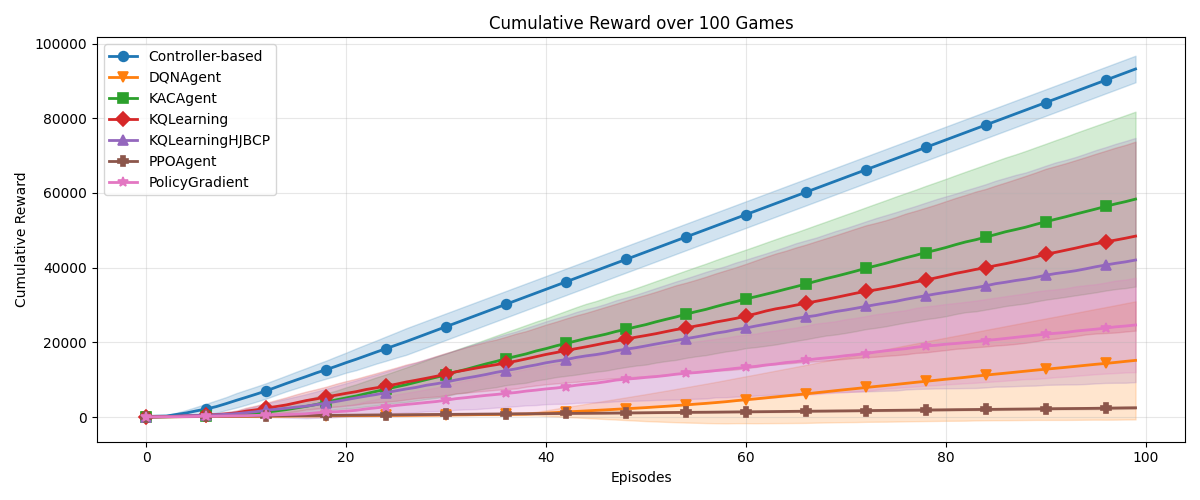
\includegraphics[width=\textwidth]{figs/plot_rewards_CP.png}
        \caption{Mean cumulative reward per episode}
        \label{fig:image1}
    \end{subfigure}
    \hfill
    \begin{subfigure}{0.48\textwidth}
        \centering
        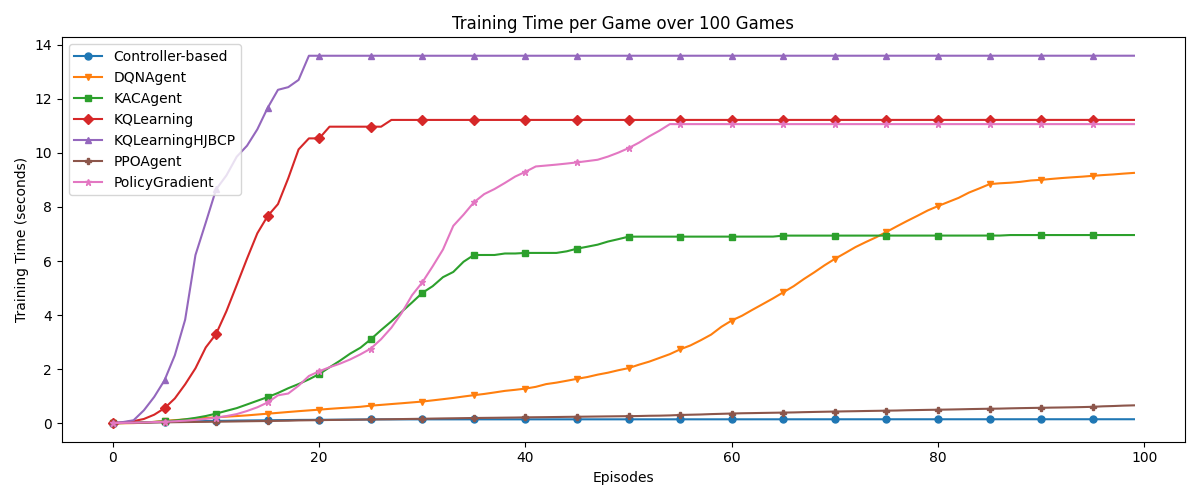
\includegraphics[width=\textwidth]{figs/plot_times_CP.png}
        \caption{Mean Cumulative time per episode}
        \label{fig:image2}
    \end{subfigure}
\end{figure}

\hypertarget{Lunar-Lander}{%
\subsection{Lunar-Lander}\label{Lunar-Lander}}


The LunarLander environment simulates the task of landing a spacecraft on a lunar surface. The agent must control the lander's thrusters to navigate it to a landing pad while minimizing fuel consumption and ensuring a safe touchdown. We considered the discrete action space LunarLander environment, defining a state space $\mathcal{S} \subset \mathbb{R}^8$ (canonical positions and speeds, angular position and speed, and two discrete flags to indicate if the pad is in contact with the ground), with four possible actions $\mathcal{A} = \{0,1,2,3\}$ (no action, fire left/right/main engine).

Data episodes are truncated to the first two thousands, and no more training occurs after 50 seconds cumulative training times.

\begin{figure}[!htb]
    \centering
    \begin{subfigure}{0.48\textwidth}
        \centering
        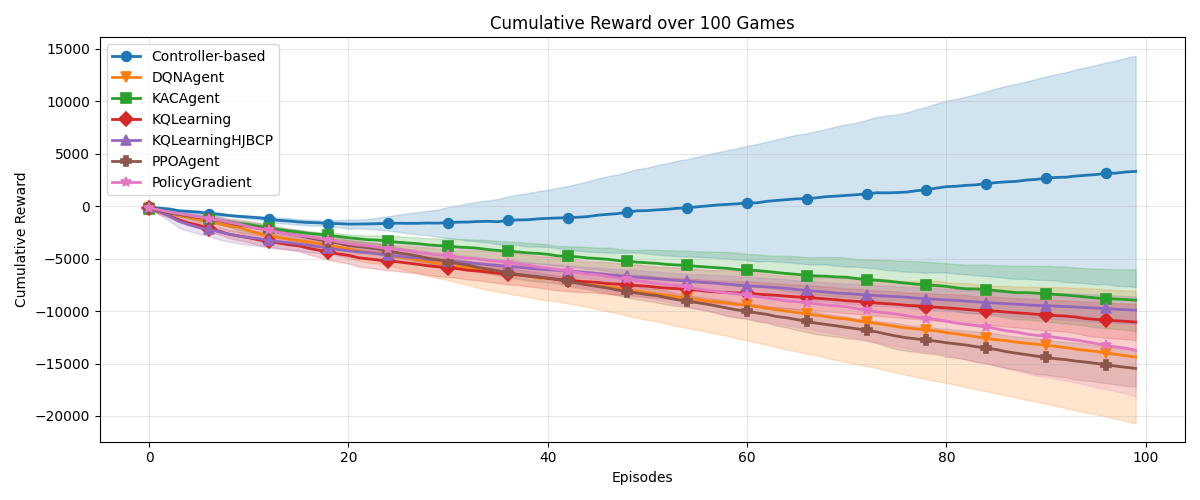
\includegraphics[width=\textwidth]{figs/plot_rewards_LN.png}
        \caption{Mean cumulative reward per episode}
        \label{fig:LNR}
    \end{subfigure}
    \hfill
    \begin{subfigure}{0.48\textwidth}
        \centering
        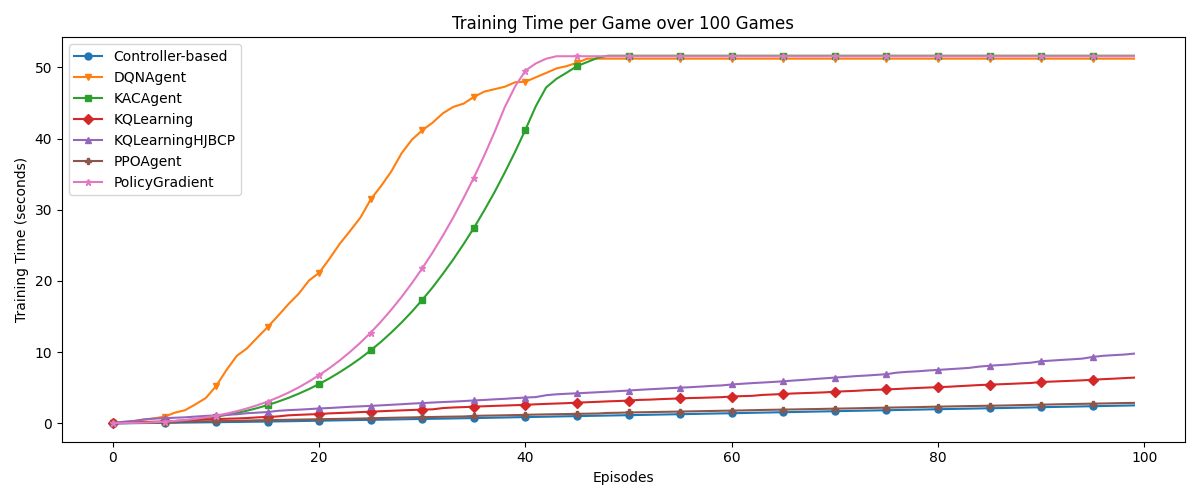
\includegraphics[width=\textwidth]{figs/plot_times_LN.png}
        \caption{Mean Cumulative time per episode}
        \label{fig:LNT}
    \end{subfigure}
\end{figure}


Among all evaluated algorithms, the heuristic-controlled learning agent achieved the highest cumulative reward, although with a large variance across episodes.  In order to achieve this result, we had to use a relatively complex controller $\mathcal{C}^{\theta}(s)$, having $12$ free parameters, see \cite{HeuristicLunar}. 


Due to non-stationary of the environment, the lunar surface is changing in each episode, value-based methods relying on Bellman error minimization such as KQLearning, KACAgent or Q-ValueGradient, and variants - face challenges in stability of learning and convergence, as noted in \cite{FuMePrNaSh} and \cite{sutton2018}. 

Similar score results to ActorCritic and Q-ValueGradient would also hold with the original KQLearning or its HJB version. Instead, we propose an episode clustered version of both algorithms, clearly enhancing training times, at the expense of scores, to illustrate scalability. This tiny modification of the original algorithm is described in annex \ref{SEK}, and can be implemented for all other flavours of residual Bellman errors based algorithms (Actor Critic, Q-ValueGradient).

\hypertarget{Conclusion}{%
\section{Conclusion}\label{Conclusion}}

We introduced a baseline of generic, scalable, sample-efficient kernel-based algorithms showing excellent raw performances as Bellman residual solvers. This framework provides a unified approach applicable in a wide range of use-cases from reinforcement learning and mathematical finance, as pricing, risk evaluation, or investment strategies.

The proposed baseline is easily extensible and opens a number of promising directions for further research and development. Notably, the future work could explore advanced exploration strategies, subsampling methods, kernel engineering as the use of convolutional kernels to deal with in-game images or videos and introducing latent spaces to deal with high-dimensional structures.

\newpage

\begin{thebibliography}{1}

\bibitem{Chowdhury2017proceedings} 
{\sc Sayak Ray Chowdhury and Aditya Gopalan}, 
{\sl On Kernelized Multi-armed Bandits.}
Proceedings of the 34th International Conference on Machine Learning, in Proceedings of Machine Learning Research - 70 , pp 844-853 

\bibitem{Cuturi:2013} 
{\sc M. Cuturi,} 
Sinkhorn distances: lightspeed computation of optimal transport, 
 Advances in Neural Information
Processing Systems 26: 27th Annual Conference on Neural Information Processing Systems 2013, C.J.C. Burges, L. Bottou, Z. Ghahramani, and K.Q. Weinberger, editors, 
Proceedings of a meeting held December 5-8, 2013, Lake Tahoe, Nevada, United States, pp. 2292--2300.


\bibitem{Mania2018} 
{\sc Mania, H., Guy, A., and Recht, B.}, 
Simple random search of
static linear policies is competitive for reinforcement learning. In Advances in Neural Information Processing Systems, 1800–1809.


\bibitem{ChengHC2021} 
{\sc Cheng, Ching-An and Kolobov, Andrey and Swaminathan, Adith}, 
{\sl Heuristic-guided reinforcement learning.}
Proceedings of the 35th International Conference on Neural Information Processing Systems - 1038, pp 13550 - 13563

\bibitem{mnih2015}{
Mnih et al. (2015)}{"Human-level control through deep reinforcement learning"
}

\bibitem{vanhasselt2016}{
Van Hasselt, Guez, \& Silver (2016) "Deep Reinforcement Learning with Double Q-learning"}

\bibitem{Reinforce} 
{\sc Williams, Ronald J.}, 
{\sl Simple statistical gradient-following algorithms for connectionist reinforcement learning}
Machine Learning, 8(3-4): pp 229-256

\bibitem{SF2023}{Sing-Yuan Yeh, Fu-Chieh Chang, Chang-Wei Yueh, Pei-Yuan Wu, Alberto Bernacchia, Sattar Vakili}{Sample Complexity of Kernel-Based Q-Learning}

\bibitem{PLF-JMM-Wilmott}
{\sc P.G. LeFloch and J.-M. Mercier,} 
Extrapolation and generative algorithms for three applications in finance,
Wilmott, vol. 2024, iss. 133, 2024.

\bibitem{codpy}
{\sc P.G. LeFloch, J.-M. Mercier, and S. Miryusupov,}
CodPy: a Python library for numerics, machine learning, and statistics.
arXiv:2402.07084


\bibitem{LeMeMi:2024}
{\sc P.G. LeFloch, J.-M. Mercier, and S. Miryusupov,}
A class of kernel-based scalable algorithms for data science. arXiv:2410.14323

\bibitem{LeMe:2017}
{\sc P.G. LeFloch, J.-M. Mercier, }
A new method for solving Kolmogorov equations in mathematical finance,
DOI : 10.1016/j.crma.2017.05.003

\bibitem{watkins1992} 
{\sc Watkins, C. J. C. H., \& Dayan, P. }, 
{\sl Q-learning.}
Machine Learning, 8(3-4), pp 279–292.

\bibitem{FuMePrNaSh} 
{\sc Watkins, C. J. C. H., \& Dayan, P. }, 
Why Should I Trust You, Bellman? The Bellman Error is a Poor Replacement for Value Error, arXiv:2201.12417 [cs.LG]
, https://doi.org/10.48550/arXiv.2201.12417


\bibitem{DQN} 
{\sc Volodymyr Mnih, Koray Kavukcuoglu,David Silver, Alex Graves, Ioannis Antonoglou, Daan Wierstra and Martin A. Riedmiller }, 
{\sl Playing Atari with Deep Reinforcement Learning.} 

\bibitem{sutton2018} 
{\sc Sutton, R. S., \& Barto, A. G.}, 
{\sl Reinforcement learning: An introduction (2nd ed.)}
MIT Press.

\bibitem{BTA}
{\sc A. Berlinet and C. Thomas-Agnan,}
{\it Reproducing kernel Hilbert spaces in probability and statistics,}
Springer Science, Business Media, LLC, 2004.

\bibitem{silver2014}
{
Silver et al. (2014) "Deterministic Policy Gradient Algorithms"
}

\bibitem{PPO} 
{\sc John Schulman, Filip Wolski, Prafulla Dhariwal, Alec Radford and Oleg Klimov}, 
{\sl Proximal Policy Optimization Algorithms}
 arXiv:1707.06347, 
https://doi.org/10.48550/arXiv.1707.06347

\bibitem{ormoneit2002}{Ormoneit, Sen}{
Kernel-Based Value Function Approximation (2002)
}

\bibitem{engel2003}{Engel et al.}{Gaussian Process Temporal Difference Learning (GPTD) (2003)}

\bibitem{Xu2007}
{\sc X. Xu, D. Hu and X. Lu,}
{\it Kernel-Based Least Squares Policy Iteration for Reinforcement Learning,}
in IEEE Transactions on Neural Networks, vol. 18, no. 4, pp. 973-992, July 2007, doi: 10.1109/TNN.2007.899161.

\bibitem{Jon2023}
Symphony of experts: orchestration with adversarial insights in
reinforcement learning
{\sc M. Jonckheere, C. Mignacco and G.Stoltz,}

2023, \url{https://arxiv.org/abs/2310.16473}

\bibitem{HeuristicLunar}
{\sc Andrea PIERRÉ}
{\it LunarLander Heuristic controller}
\url{https://github.com/openai/gym/blob/master/gym/envs/box2d/lunar_lander.py}, Line 726. 


\bibitem{DLR1}
{\sc A.-M. Leventi-Peetz, T. Östreich}
Deep Learning Reproducibility and Explainable AI (XAI)
{\it arXiv preprint: arXiv:2202.11452v3}

\bibitem{DLR2}
{\sc Peter Henderson, Riashat Islam, Philip Bachman, Joelle Pineau, Doina Precup, David Meger}
Deep Reinforcement Learning that Matters
{\it arXiv preprint  arXiv:1709.06560v3}

\bibitem{DLR3}
{\sc Biao Xu, Guanci Yang}
Interpretability research of deep learning: A literature survey
{\it Information Fusion, Volume 115, 2025}

\bibitem{DLR4}
{\sc Aparna Balagopalan, Haoran Zhang, Kimia Hamidieh, Thomas Hartvigsen, Frank Rudzicz, Marzyeh Ghassemi}
The Road to Explainability is Paved with Bias: Measuring the Fairness of Explanations
{\it arXiv preprint arXiv:2205.03295v2}

\bibitem{DLR5}
{\sc Kumar, Rishab \& Koshiyama, Adriano \& da Costa, Kleyton \& Kingsman, Nigel \& Kazim, Emre \& Roy, Arunita \& Treleaven, Philip \& Lovell, Zac. (2023).}
Deep learning model fragility and implications for financial stability and regulation. 
{\it Bank of England, Staff Working Paper No. 1,038}

\end{thebibliography}

\appendix
\hypertarget{APPENDIX}{%
\section{APPENDIX}\label{APPENDIX}}

\subsection{The softmax function}

We recall that the softmax function, used to any map any vector
\(y=(y^1,\dots,y^{|\mathcal{A}|})\) to a vector of probabilities
\(\pi=(\pi^1,\dots,\pi^{|\mathcal{A}|})\), is characterized as
\begin{equation} \label{eq:softmax}
 \text{softmax}(y) = \frac{\exp(y^i)}{\sum_{j=1}^{|\mathcal{A}|} \exp(y^j)}=\pi, \quad \frac{\partial}{\partial y^j}\text{softmax}(y^i) = \pi^i(\delta^i(j)-\pi^j).
\end{equation}
The softmax pseudo-inverse is defined as
\(y=\ln \pi\)

\hypertarget{SEK}{%
\subsection{A clustering methodology using kernel baseline RL algorithms}
\label{SEK}
}

Clustering is a natural and efficient strategy to reduce computation burden of kernel methods. The general idea is to define a partition of the buffer $B^{T} = \{(s_t, a_t, s_{t}', r_t, d_t) \}_{t=1}^{T}$ into $I$ clusters $B_i^{T} = \{(s_t^i, a_t^i, s_{t}'^i, r_t^i, d_t^i) \}_{t=1..T^i}$. Each cluster is associated with a local agent $\mathcal{A}_i, i = 1, \dots, I$, which independently solves the Bellman equation \eqref{eq:bel_res}, using its own kernel $k_i$. While this approach is conceptually similar to the \textit{symphony of experts} \cite{Jon2023}, our approach differs technically as described below.

A simple and efficient method is to associate each in-game episode with a distinct cluster. For each cluster we solve the optimal Bellman equation as in section \ref{Kernel Q-Learning}, or its HJB counterpart \ref{KHJB}, and denote its local value function $q_{k_i}^*(\cdot)$. This episodic clustering is well adapted to the LunarLander game, where episodes usually contains a small number of 100-200 steps, allowing fast and competitive learning times, as shown in picture \ref{fig:LNT}. Importantly, we found that using cluster specific local gamma values improves performance. In our experiments, we set the following $\gamma^i=\exp(-\frac{-\ln(T^i)}{T^i})$. 

Each agents naturally induces a distance metric which is based on its associated experience buffer. Given a state-space action pair $z = (s,a)$, we define distance  to the buffer used by each agent $\mathcal{A}_i$:
$$
d(z,\mathcal{A}_i) = d_i(z,z^{i^*(s)}), \quad i^*(s) = \arg \inf_i d_i(z,Z_i), z=s,a, \ \quad Z_i = \{s_t^i, a_t^i\}_{t= 1 \ldots T^i},
$$
where $d_i(\cdot,\cdot)$ is a distance function. A natural choice for kernel methods is to pick-up the kernel discrepancy as a distance, $d_i(x,y) = k_i(x,x)+k_i(y,y) - 2 k_i(x,y)$, that is the distance selected for our experiments.

During a gameplay, given a current state $s$, we select the action $\arg \max_{a=1,..,|\mathcal{A}|} q^*(s,a)$, where the optimal state value function $q^*(s,a)$ is approximated as follows. We first identify the closest $I \times |\mathcal{A}|$ points to $s,a$, denoted $X = \{s_{i^*(s)},a_{i^*(s)}\}_i$, 
along with their local optimal q-values denoted $Y = \{q_i(s_{i^*(s)},a_{i^*(s)})\}$. These values $(X,Y)$ are then extrapolated in order to provide a value $q_k^*(s,a)$. In the context of reinforcement learning, we used the transition formula \eqref{cond} $q^*(s,a) \sim \tau_k^{Y | X}(s,a)$ in order to provide an extrapolation mechanism of these in-game agent data.

\hypertarget{SEK}{%
\subsection{PPO under Standard Training Protocol}
\label{PPO_app}
}
Section \ref{Lunar-Lander} showed that under tight training constraints, specifically, a limited number of episodes and a cumulative time budget of 50 seconds on learning-based agents. This setup emphasizes sample efficiency but diverge from standard practices in reinforcement learning, where algorithms are usually allowed to have extended interaction with the environment. To better understand learning dynamics and insure fair comparison, we repeated our experiments under more standard PPO conditions, while keeping the cap of 50 seconds. It allowed to explore PPO's sample efficiency more aptly, while remaining cautious in our interpretations, since its performance improve with increased number of interactions with environment. 


\begin{figure}[!htb]
    \centering
    \begin{subfigure}{0.48\textwidth}
        \centering
        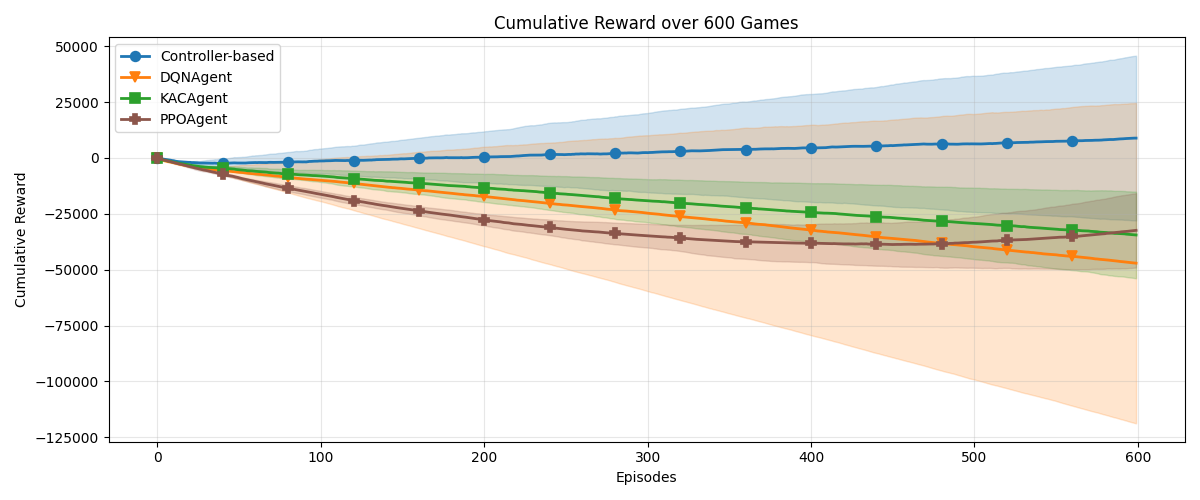
\includegraphics[width=\textwidth]{figs/plot_rewards.png}
        \caption{Mean cumulative reward per episode}
        \label{fig:PPOLNR}
    \end{subfigure}
    \hfill
    \begin{subfigure}{0.48\textwidth}
        \centering
        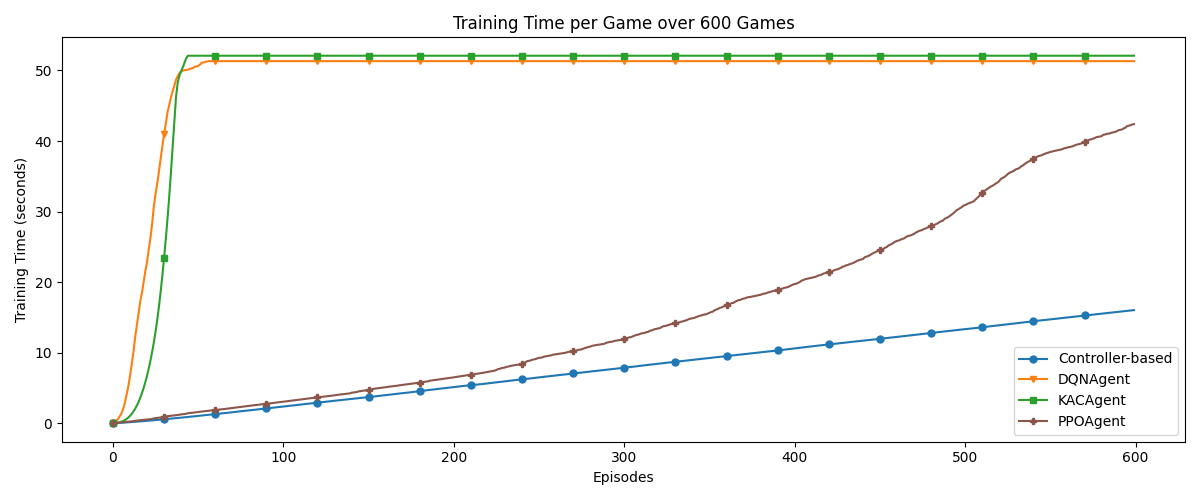
\includegraphics[width=\textwidth]{figs/plot_times.png}
        \caption{Mean Cumulative time per episode}
        \label{fig:PPOLNT}
    \end{subfigure}
\end{figure}


Figure \ref{fig:PPOLNR} shows mean cumulative rewards obtained by all agents over 600 episodes. While the PPO agent starts under-performing, this early decline in cumulative rewards is expected. PPO begins an initial exploration phase, where it gains diverse experience through interaction with an environment. This phase is suboptimal especially when time or samples are limited. However we note that closer to 600-th episode the PPO is reversing its trend, showing a steady improvement in reward. This behaviour demonstrates PPO's dependence on rich environmental feedback and longer training horizons.  


\end{document}